\documentclass[10pt]{article}
\usepackage[letterpaper,textwidth=5.5in,textheight=9in,top=1in,headsep=0.25in,footskip=0.4in]{geometry}
\usepackage[T1]{fontenc}\usepackage[utf8]{inputenc}\usepackage{lmodern}\usepackage{microtype}
\usepackage{amsmath,amssymb}\usepackage{makecell,booktabs,graphicx,xcolor,enumitem,float}
\usepackage[numbers,square,sort&compress]{natbib}
\usepackage[font=small,labelfont=bf,labelsep=colon,skip=6pt]{caption}
\usepackage{titlesec}
\titleformat{\section}{\large\bfseries}{\thesection}{0.6em}{}
\titleformat{\subsection}{\normalsize\bfseries}{\thesubsection}{0.6em}{}
\titlespacing*{\section}{0pt}{12pt plus 2pt minus 2pt}{6pt}
\titlespacing*{\subsection}{0pt}{9pt plus 2pt minus 2pt}{4pt}
\setlength{\emergencystretch}{1.5em}\setlength{\parindent}{0pt}\setlength{\parskip}{5.5pt}
\definecolor{mydarkblue}{rgb}{0,0.08,0.45}
\usepackage[colorlinks=true,linkcolor=mydarkblue,citecolor=mydarkblue,urlcolor=mydarkblue]{hyperref}
\setlist{itemsep=1pt,topsep=2pt,leftmargin=1.5em}
\renewcommand{\paragraph}[1]{\textbf{#1}\hspace{0.5em}}
\begin{document}
\thispagestyle{plain}
\begin{center}
\rule{\linewidth}{4pt}\par\vspace{0.18in}
{\LARGE\bfseries HARVI-ECG: Heart-Failure Readouts from a\\[2pt] 10-Second 12-Lead ECG\par}
\vspace{0.12in}\rule{\linewidth}{1pt}\par\vspace{0.22in}
{\bfseries Medical University of Vienna}\\
Center for Medical Physics and Biomedical Engineering\par
\vspace{0.2in}
\end{center}
\begin{center}{\large\bfseries Abstract}\end{center}\vspace{-4pt}
\begin{quote}\small
HARVI-ECG turns a standard 10-second 12-lead ECG into heart-failure readouts. It is built on an ECG foundation encoder pretrained without labels on 6{,}009{,}279 ECGs from 3{,}257{,}195 patients, and provides two readouts: an \emph{NT-proBNP readout} (an NT-proBNP estimate with rule-out, age-adjusted rule-in and severe decisions) and a \emph{structural heart disease (SHD) module} that detects echo-defined structural heart disease. On MIMIC-IV (18{,}036 ECG--NT-proBNP pairs, 11{,}929 patients, patient-grouped 5-fold cross-validation), the NT-proBNP readout reached a mean rule-out/rule-in AUROC of 0.894 (0.889--0.898) and a rule-out AUROC of 0.920 (0.914--0.925). Without retraining it transferred to two hospitals it had never seen: at Emory it detected HFrEF with AUROC 0.810 (0.803--0.816) and HFpEF with 0.727 (0.719--0.735) against age- and sex-matched controls, and at EchoNext it identified echocardiographic reduced ejection fraction with AUROC 0.834. HARVI-ECG outperformed a task-specific baseline trained from scratch, most clearly at the unseen hospital (Emory HFrEF +0.036 (+0.031 to +0.040), HFpEF +0.055 (+0.049 to +0.060)). Adapted on EchoNext echocardiography labels, the SHD module reached AUROC 0.929 for reduced ejection fraction and 0.850 for composite structural heart disease on held-out patients, and needed only 250 labelled patients to match the zero-label NT-proBNP readout for LVEF $\le$45\,\%.
\end{quote}
\vspace{2pt}
\begin{figure}[h]\centering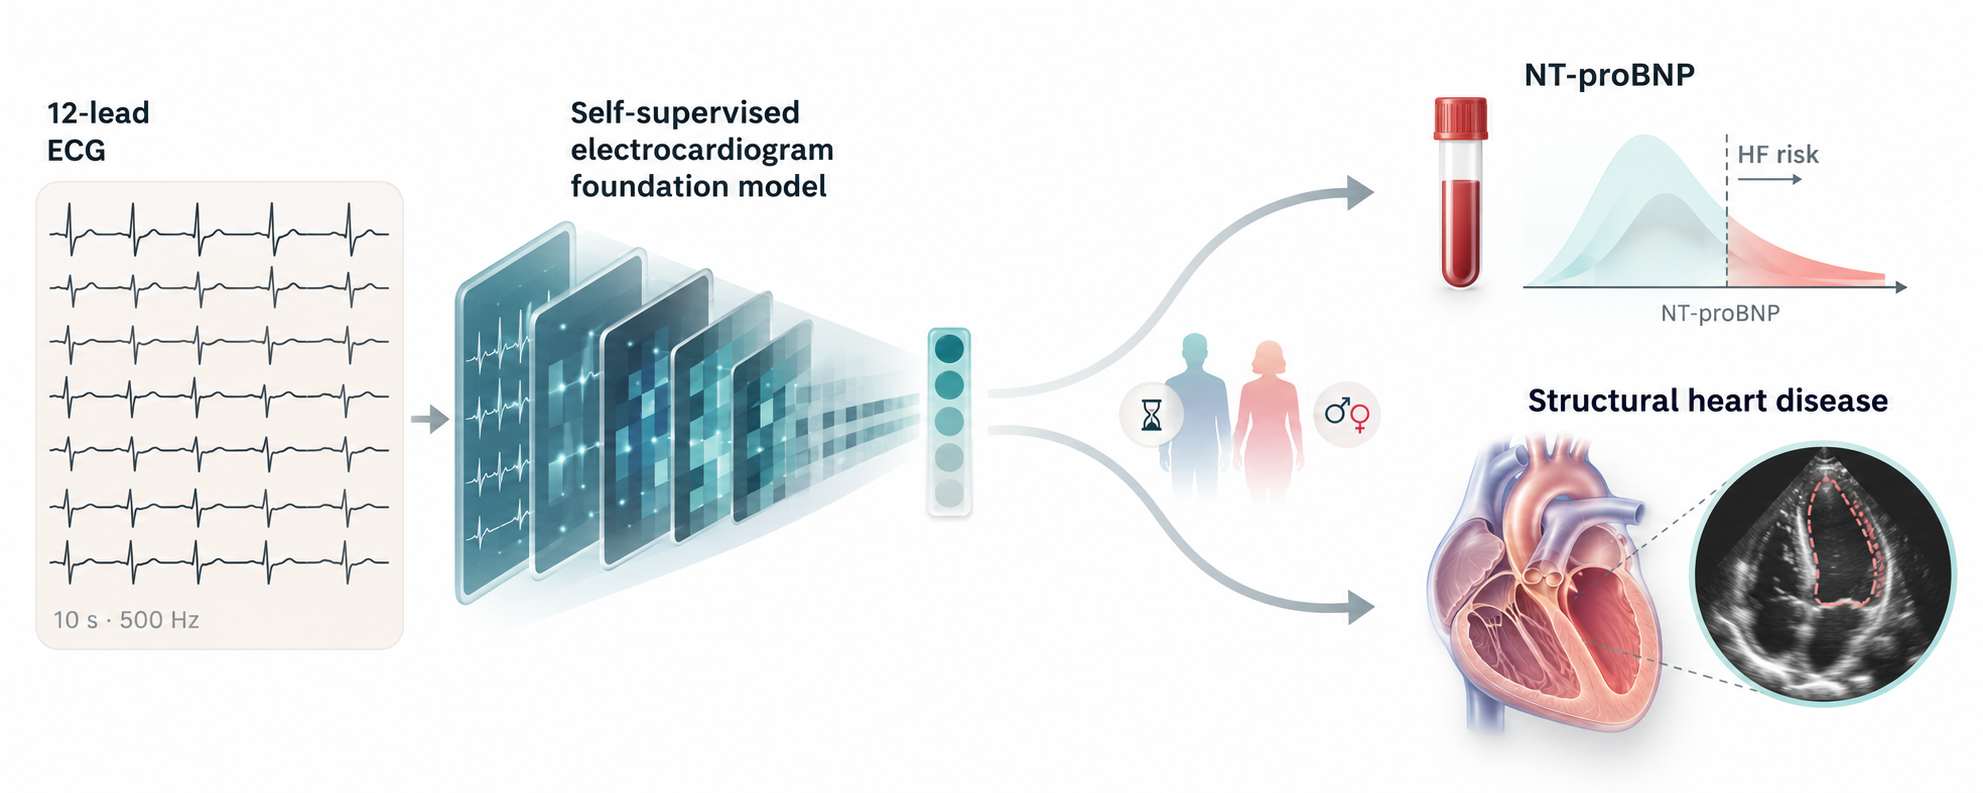
\includegraphics[width=\linewidth]{harvi_visual_abstract.png}
\caption*{\small\textbf{Overview.} A 10-second 12-lead ECG is encoded by a self-supervised ECG foundation model; HARVI-ECG reads out NT-proBNP-based heart-failure risk and echo-defined structural heart disease.}\end{figure}
\renewcommand{\thefootnote}{}\footnotetext{Technical report v1.3, October 2026. Code: \url{https://github.com/CellularSyntax/harvi-ecg-eval}. Archive: \href{https://doi.org/10.5281/zenodo.23367346}{doi:10.5281/zenodo.23367346}. Model weights (on request): \url{https://huggingface.co/maxhaberbusch/HARVI-ECG}.}\renewcommand{\thefootnote}{\arabic{footnote}}

\section{Model}\label{sec:model}
\begin{figure}[t]\centering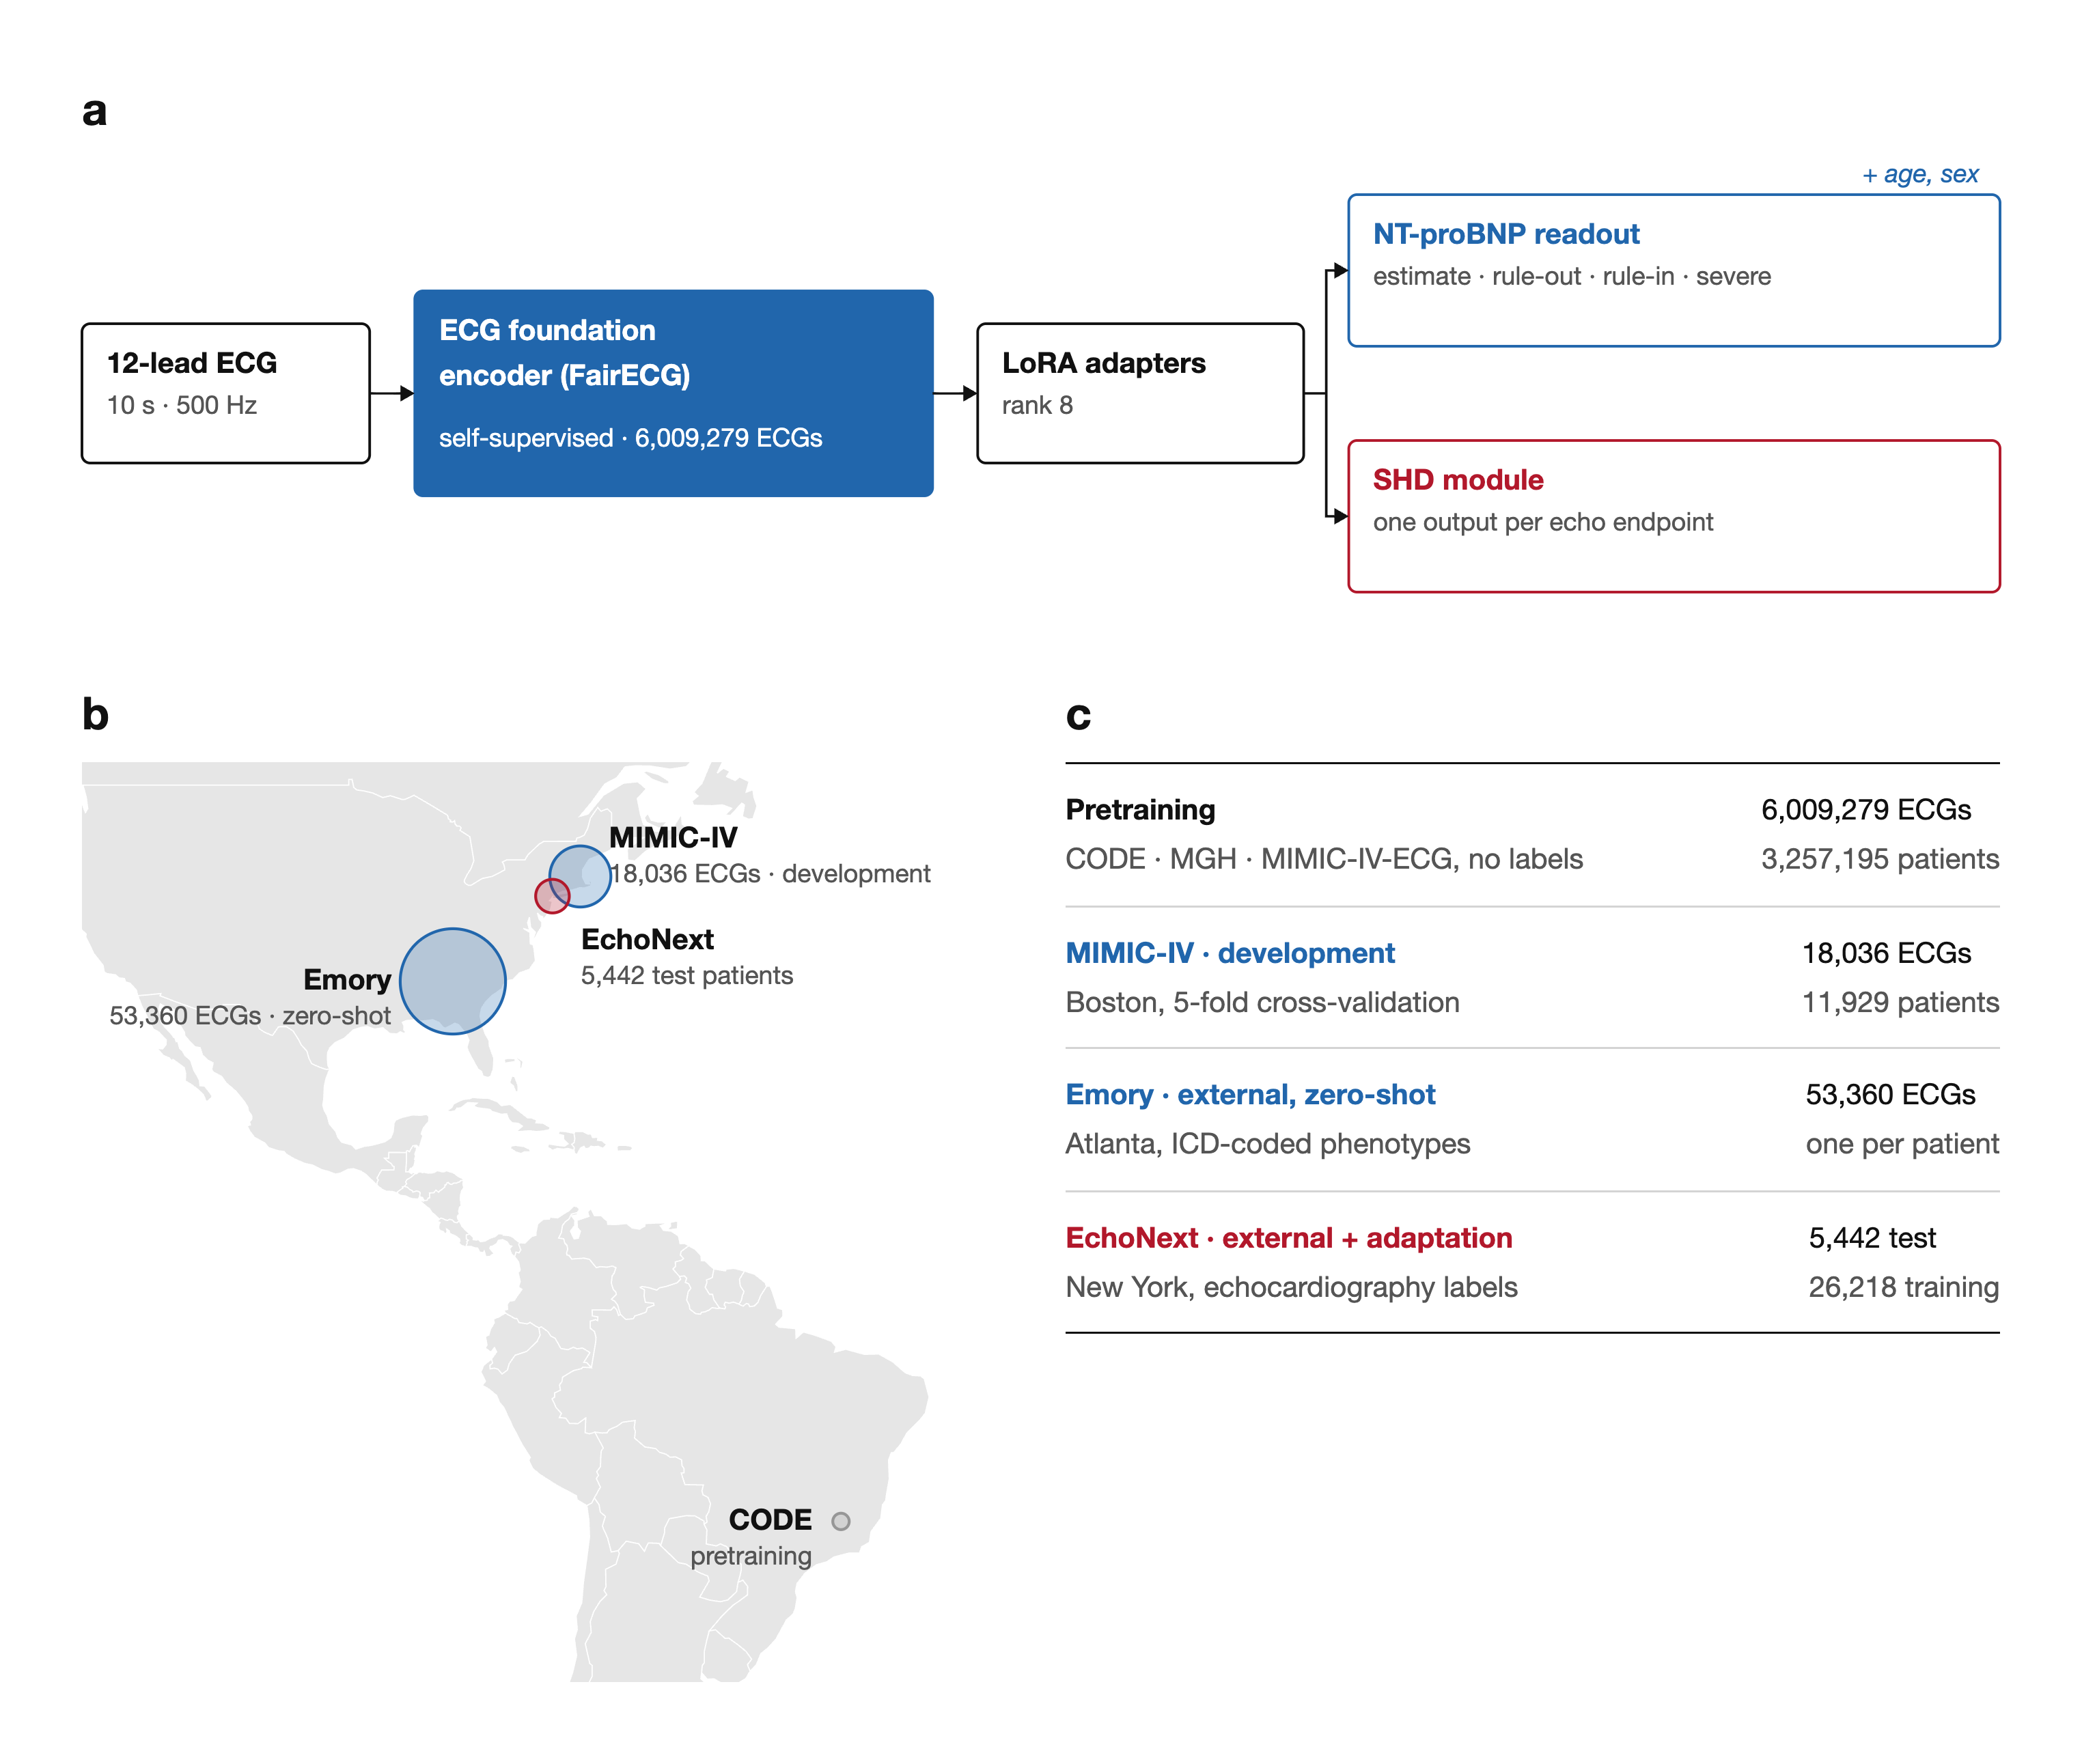
\includegraphics[width=\linewidth]{harvi_fig1_overview.png}
\caption{HARVI-ECG and its cohorts. (a) Architecture; age and sex feed only the NT-proBNP readout. (b) Cohort sites; circle area is proportional to cohort size. The Boston circle marks MIMIC-IV; the pretraining sources MGH and MIMIC-IV-ECG are also Boston-based and are listed in (c). (c) Cohort roles and counts. Emory and EchoNext were used neither in pretraining nor in developing the NT-proBNP readout.}\label{fig:overview}\end{figure}
HARVI-ECG (Figure~\ref{fig:overview}a) has three parts.
\begin{itemize}
\item \textbf{ECG foundation encoder.} The FairECG encoder (internal, ongoing unpublished work), an xLSTM-based model~\cite{beck2024} pretrained with self-supervision (SimDINO) on 6{,}009{,}279 ECGs from 3{,}257{,}195 patients (CODE, MGH, MIMIC-IV-ECG; waveforms only, no labels). It maps a 10-second, 500-Hz, 12-lead ECG (each lead instance-normalised) to a 1{,}024-dimensional embedding.
\item \textbf{NT-proBNP readout.} The encoder is adapted with low-rank adapters (LoRA, rank 8)~\cite{hu2022} and feeds a shared head that also receives age and sex. The head outputs an NT-proBNP estimate with uncertainty and three guideline decisions: rule-out ($<$300\,pg/mL), age-adjusted rule-in ($>$450/900/1{,}800\,pg/mL for $<$50/50--75/$>$75 years) and severe ($>$3{,}000\,pg/mL). It is trained on MIMIC-IV only; the epoch is selected on an inner 10\,\% of training patients.
\item \textbf{SHD module.} The same encoder with LoRA and one logistic output per echocardiographic endpoint, adapted on the echo-labelled patients of a site (here EchoNext).
\end{itemize}
A task-specific baseline (ConvNeXt-1D + xLSTM with age and sex conditioning, trained from scratch on the same MIMIC-IV folds) serves as a reference (Section~\ref{sec:found}); because it also differs in architecture, training recipe and checkpoint selection, the comparison does not isolate the effect of pretraining alone. Analyses followed pre-specifications fixed before scoring; the primary decision metric was the mean of the rule-out and rule-in AUROCs, with 95\,\% CIs from a 2{,}000-draw patient bootstrap.

\section{Data}\label{sec:data}
\paragraph{MIMIC-IV (development).} 18{,}036 ECG--NT-proBNP pairs from 11{,}929 patients of the MIMIC-IV-ECG matched subset~\cite{gow2023,johnson2023}. Median age 72 years (IQR 60--82); 50.4\,\% female; NT-proBNP median 2{,}046\,pg/mL (IQR 515--6{,}276). Prevalence: rule-out 18.1\,\%, rule-in 61.6\,\%, severe 41.1\,\%. Folds are \texttt{GroupKFold(5)} on patient.

\paragraph{Emory (external).} Site I0006 of the Harvard-Emory ECG Database~\cite{koscova2026}, used neither for development nor for pretraining. HFrEF (ICD-10 I50.2x) and HFpEF (I50.3x) cases, with the ECG closest to the first subtype code ($-$180 to $+$30 days), against controls without any I50 code and at least 365 days of follow-up, matched 4:1 on sex and 5-year age band. HFrEF: 5{,}627 cases, 22{,}508 controls. HFpEF: 5{,}045 cases, 20{,}180 controls. One ECG per patient (53{,}360 in total). The stored aVL and aVF channels were rebuilt from leads I and II before scoring.

\paragraph{EchoNext (external).} 12-lead ECGs paired with transthoracic echocardiography (Columbia University), with patient-disjoint training, validation and test splits; not used in pretraining. All EchoNext results refer to the 5{,}442 test patients (one ECG each). Endpoints: composite structural heart disease (moderate or greater, EchoNext definition), LVEF $\le$45\,\%, LV wall thickness $\ge$13\,mm and reduced ejection fraction (LVEF $\le$40\,\% vs $\ge$50\,\%; post hoc).

\section{NT-proBNP readout}\label{sec:ntp}
\begin{figure}[p]\centering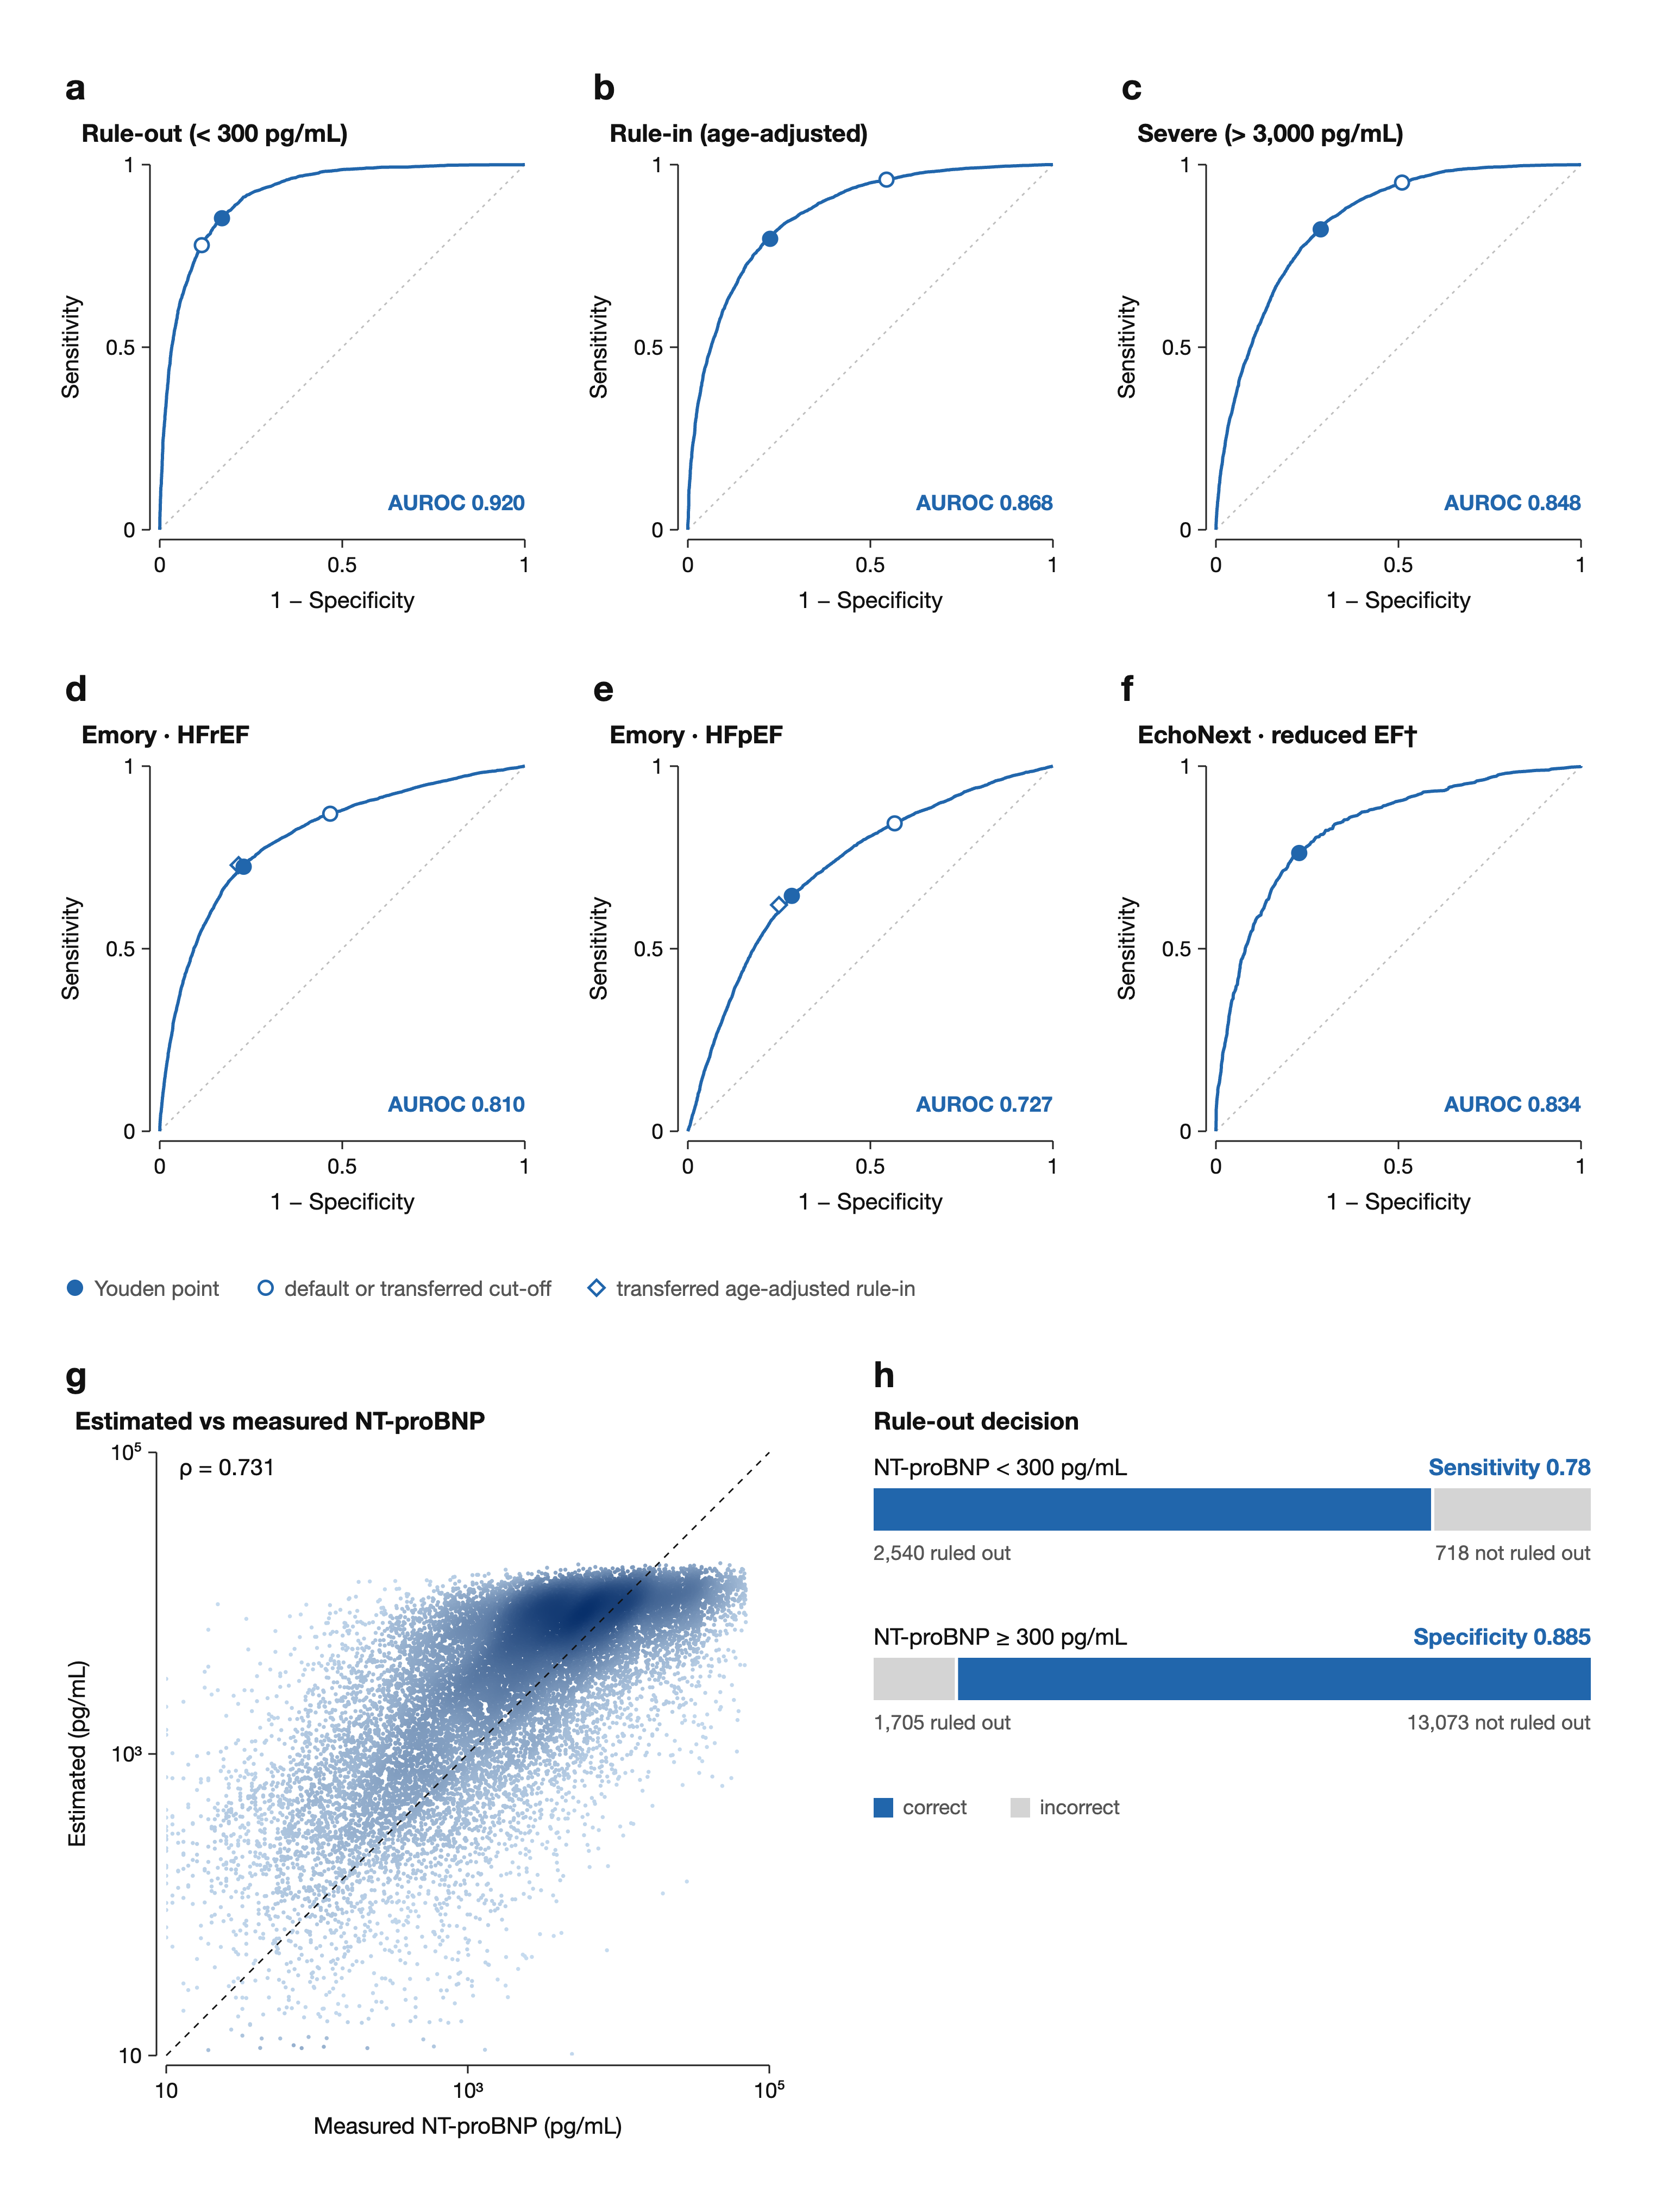
\includegraphics[width=\linewidth]{harvi_fig2_ntprobnp.png}
\caption{NT-proBNP readout. (a--c) MIMIC-IV out-of-fold ROC curves for rule-out ($<$300\,pg/mL), age-adjusted rule-in and severe ($>$3{,}000\,pg/mL). (d, e) Emory, zero-shot: ICD-coded HFrEF and HFpEF against age- and sex-matched controls. (f) EchoNext held-out test patients, reduced EF$^\dagger$, zero-shot. Filled circles: Youden points with thresholds chosen on separate data (Section~\ref{sec:ops}); open circles: default (head probability $\geq$0.5) or transferred 300\,pg/mL cut-off; open diamonds: transferred age-adjusted rule-in cut-offs. (g) Estimated versus measured NT-proBNP per ECG, coloured by density (log axes; ECGs with estimates at the 10\,pg/mL floor not shown; dashed: line of identity). (h) Rule-out decision at the default operating point; positive class = measured NT-proBNP $<$300\,pg/mL. $^\dagger$LVEF $\le$40\,\% vs $\ge$50\,\%, post hoc.}\label{fig:ntp}\end{figure}
\paragraph{Development.} On MIMIC-IV, HARVI-ECG reached AUROC 0.920 (0.914--0.925) for rule-out, 0.868 (0.862--0.874) for rule-in and 0.848 (0.841--0.855) for the severe decision; the mean of rule-out and rule-in was 0.894 (0.889--0.898) (Table~\ref{tab:int}, Figure~\ref{fig:ntp}a--c). The estimate ranks patients consistently with measured NT-proBNP (Spearman $\rho$ = 0.731; Figure~\ref{fig:ntp}g). At the default operating point, the rule-out decision has sensitivity 0.780 and specificity 0.885 (Figure~\ref{fig:ntp}h). 9{,}506 of the 11{,}929 patients had ECG waveforms in the pretraining corpus; on the 2{,}423 patients without, the mean rule-out/rule-in AUROC was 0.897 (0.887--0.907) (Table~\ref{tab:unexp}).

\begin{table}[t]\centering\small\setlength{\tabcolsep}{4pt}
\caption{MIMIC-IV out-of-fold results, all patients ($n$ = 18{,}036 ECGs, 11{,}929 patients). AUROC with 95\,\% patient-bootstrap CI (2{,}000 draws). $\Delta$ is the paired difference to the task-specific baseline on the pre-specified decision metric.}\label{tab:int}
\begin{tabular}{@{}lccccc@{}}\toprule
Model & \makecell{Rule-out\\$<$300} & \makecell{Rule-in\\(age-adj.)} & \makecell{Severe\\$>$3{,}000} & \makecell{Mean rule-out\\+ rule-in} & \makecell{$\Delta$ mean vs\\baseline} \\\midrule
Task-specific baseline & \makecell{0.902\\ {\scriptsize 0.896--0.908}} & \makecell{0.863\\ {\scriptsize 0.856--0.869}} & \makecell{0.863\\ {\scriptsize 0.856--0.869}} & \makecell{0.882\\ {\scriptsize 0.877--0.888}} & --- \\ \addlinespace[2pt]
\textbf{HARVI-ECG} & \makecell{0.920\\ {\scriptsize 0.914--0.925}} & \makecell{0.868\\ {\scriptsize 0.862--0.874}} & \makecell{0.848\\ {\scriptsize 0.841--0.855}} & \makecell{0.894\\ {\scriptsize 0.889--0.898}} & \makecell{+0.011\\ {\scriptsize +0.007 to +0.015}} \\ \addlinespace[2pt]
\bottomrule\end{tabular}\end{table}

\begin{table}[t]\centering\small\setlength{\tabcolsep}{4pt}
\caption{MIMIC-IV out-of-fold results, patients whose ECGs were not in the pretraining corpus ($n$ = 3{,}674 ECGs, 2{,}423 patients). AUROC with 95\,\% patient-bootstrap CI (2{,}000 draws). $\Delta$ is the paired difference to the task-specific baseline on the pre-specified decision metric.}\label{tab:unexp}
\begin{tabular}{@{}lccccc@{}}\toprule
Model & \makecell{Rule-out\\$<$300} & \makecell{Rule-in\\(age-adj.)} & \makecell{Severe\\$>$3{,}000} & \makecell{Mean rule-out\\+ rule-in} & \makecell{$\Delta$ mean vs\\baseline} \\\midrule
Task-specific baseline & \makecell{0.900\\ {\scriptsize 0.887--0.913}} & \makecell{0.864\\ {\scriptsize 0.849--0.878}} & \makecell{0.867\\ {\scriptsize 0.853--0.880}} & \makecell{0.882\\ {\scriptsize 0.871--0.893}} & --- \\ \addlinespace[2pt]
\textbf{HARVI-ECG} & \makecell{0.924\\ {\scriptsize 0.912--0.934}} & \makecell{0.871\\ {\scriptsize 0.857--0.884}} & \makecell{0.851\\ {\scriptsize 0.836--0.866}} & \makecell{0.897\\ {\scriptsize 0.887--0.907}} & \makecell{+0.015\\ {\scriptsize +0.007 to +0.024}} \\ \addlinespace[2pt]
\bottomrule\end{tabular}\end{table}


\paragraph{Unseen hospitals.} Applied unchanged, the NT-proBNP estimate detected HFrEF at Emory with AUROC 0.810 (0.803--0.816) and HFpEF with 0.727 (0.719--0.735) (Table~\ref{tab:ext}, Figure~\ref{fig:ntp}d,e). At EchoNext it identified reduced ejection fraction with AUROC 0.834 and LVEF $\le$45\,\% with 0.830 (Figure~\ref{fig:ntp}f). How the fixed pg/mL cut-offs transfer is analysed in Section~\ref{sec:ops}.

\begin{table}[t]\centering\small\setlength{\tabcolsep}{4pt}
\caption{Zero-shot results at Emory (score: NT-proBNP estimate, mean of the five fold models). Sensitivity and specificity at the fixed MIMIC-IV cut-offs (300\,pg/mL and age-adjusted rule-in).}\label{tab:ext}
\begin{tabular}{@{}llcccc@{}}\toprule
Endpoint & Model & \makecell{AUROC\\(95\,\% CI)} & \makecell{$\Delta$ vs\\baseline} & \makecell{Sens / spec\\at 300} & \makecell{Sens / spec\\at rule-in} \\\midrule
HFrEF vs controls & Baseline & \makecell{0.774\\ {\scriptsize 0.767--0.781}} & --- & 0.98 / 0.11 & 0.89 / 0.47 \\
 & \textbf{HARVI-ECG} & \makecell{0.810\\ {\scriptsize 0.803--0.816}} & \makecell{+0.036\\ {\scriptsize +0.031 to +0.040}} & 0.87 / 0.53 & 0.73 / 0.78 \\
\addlinespace
HFpEF vs controls & Baseline & \makecell{0.672\\ {\scriptsize 0.664--0.680}} & --- & 0.98 / 0.07 & 0.81 / 0.43 \\
 & \textbf{HARVI-ECG} & \makecell{0.727\\ {\scriptsize 0.719--0.735}} & \makecell{+0.055\\ {\scriptsize +0.049 to +0.060}} & 0.84 / 0.43 & 0.62 / 0.75 \\
\bottomrule\end{tabular}\end{table}

\section{Comparison with a task-specific baseline}\label{sec:found}
\begin{figure}[t]\centering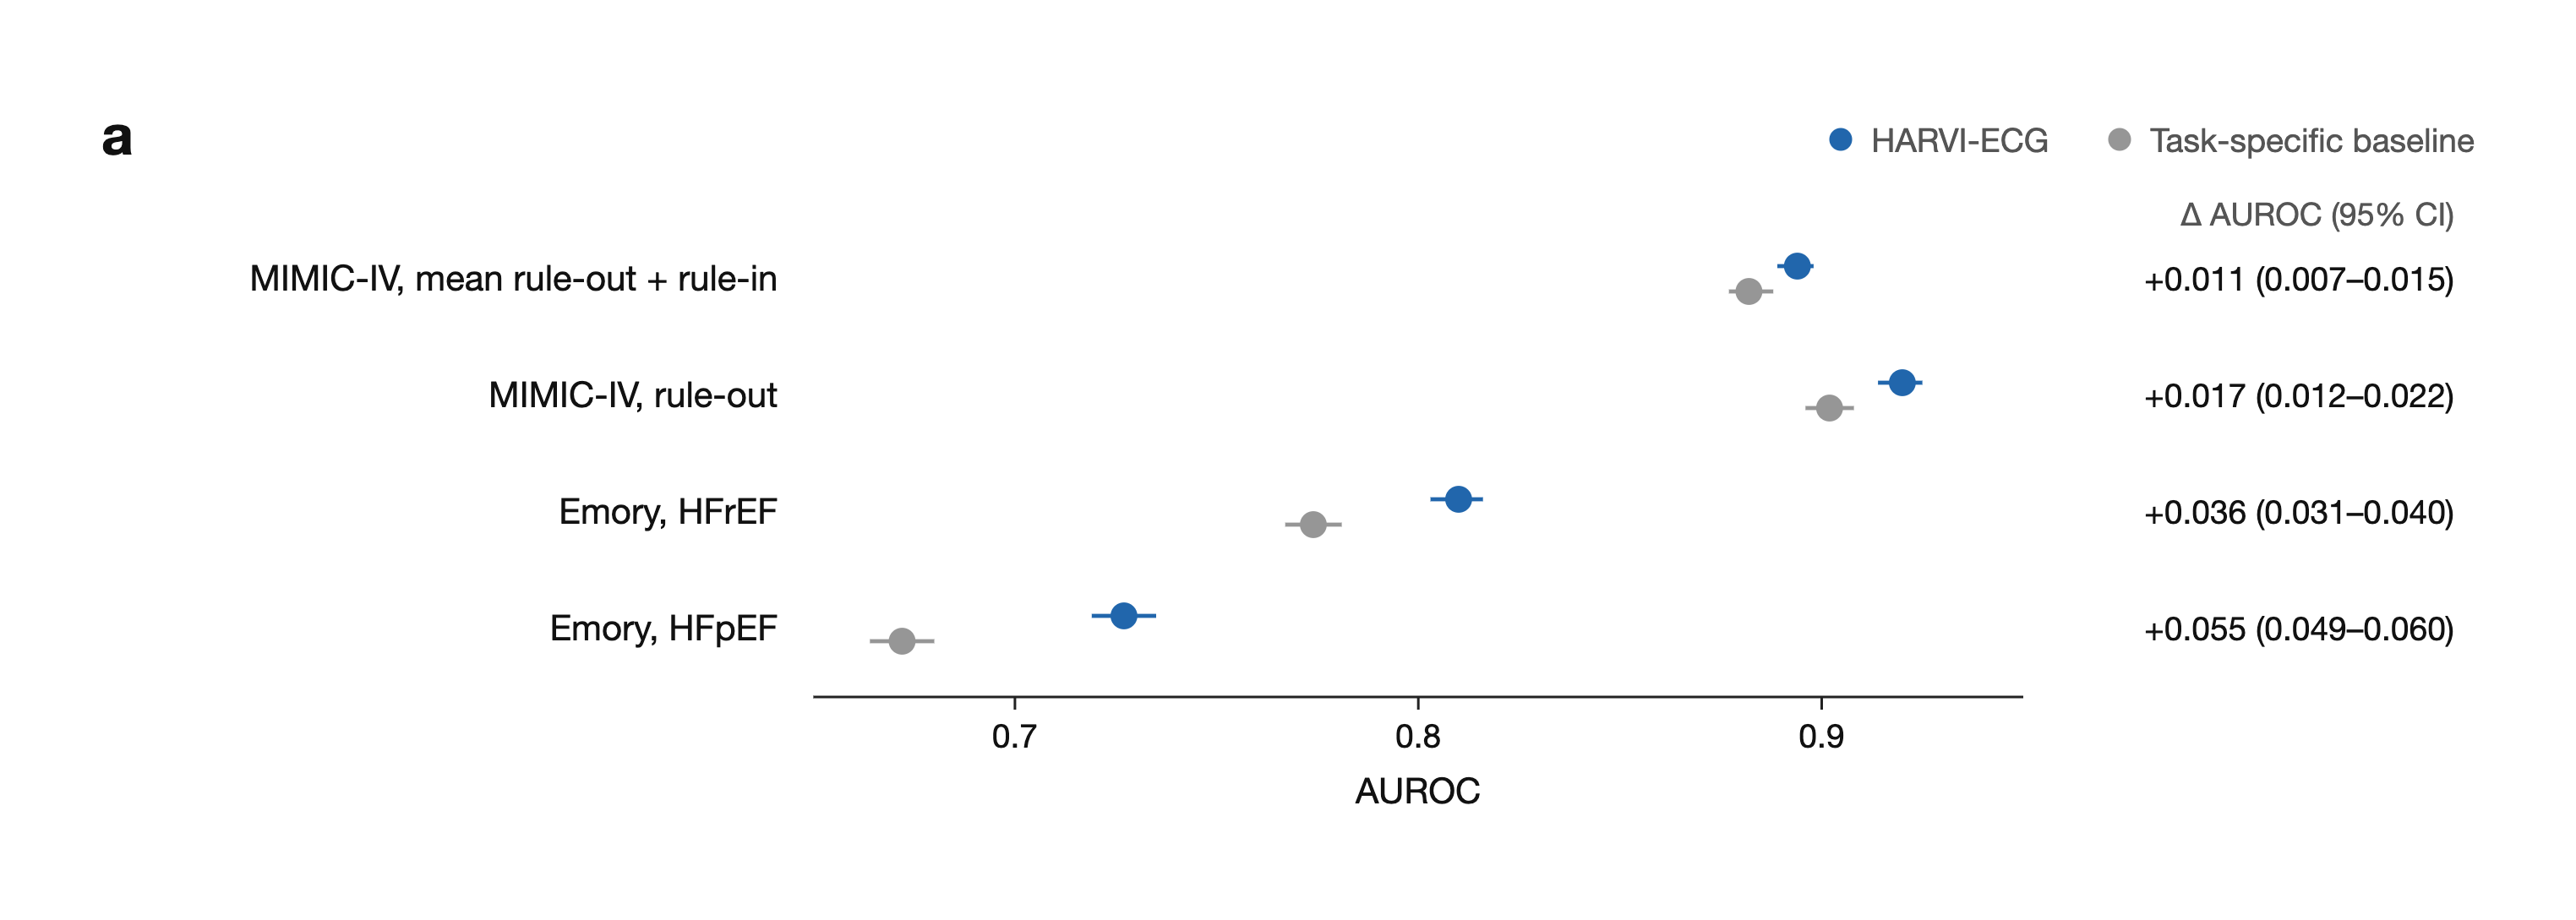
\includegraphics[width=\linewidth]{harvi_fig3_foundation.png}
\caption{HARVI-ECG against the task-specific baseline (trained from scratch on the same MIMIC-IV folds), on identical patients. AUROC with 95\,\% patient-bootstrap CI; right column: paired $\Delta$AUROC (95\,\% CI).}\label{fig:found}\end{figure}
Under the pre-specified rule, HARVI-ECG improved the mean rule-out/rule-in AUROC over the task-specific baseline by +0.011 (+0.007 to +0.015), with the CI excluding zero (Figure~\ref{fig:found}, Table~\ref{tab:int}). The gain was largest at the unseen hospital: Emory HFrEF +0.036 (+0.031 to +0.040) and HFpEF +0.055 (+0.049 to +0.060). The baseline could not be applied at EchoNext, whose waveforms are released per-lead standardised; HARVI-ECG normalises each lead itself and is unaffected.

\section{SHD module}\label{sec:shd}
\begin{figure}[t]\centering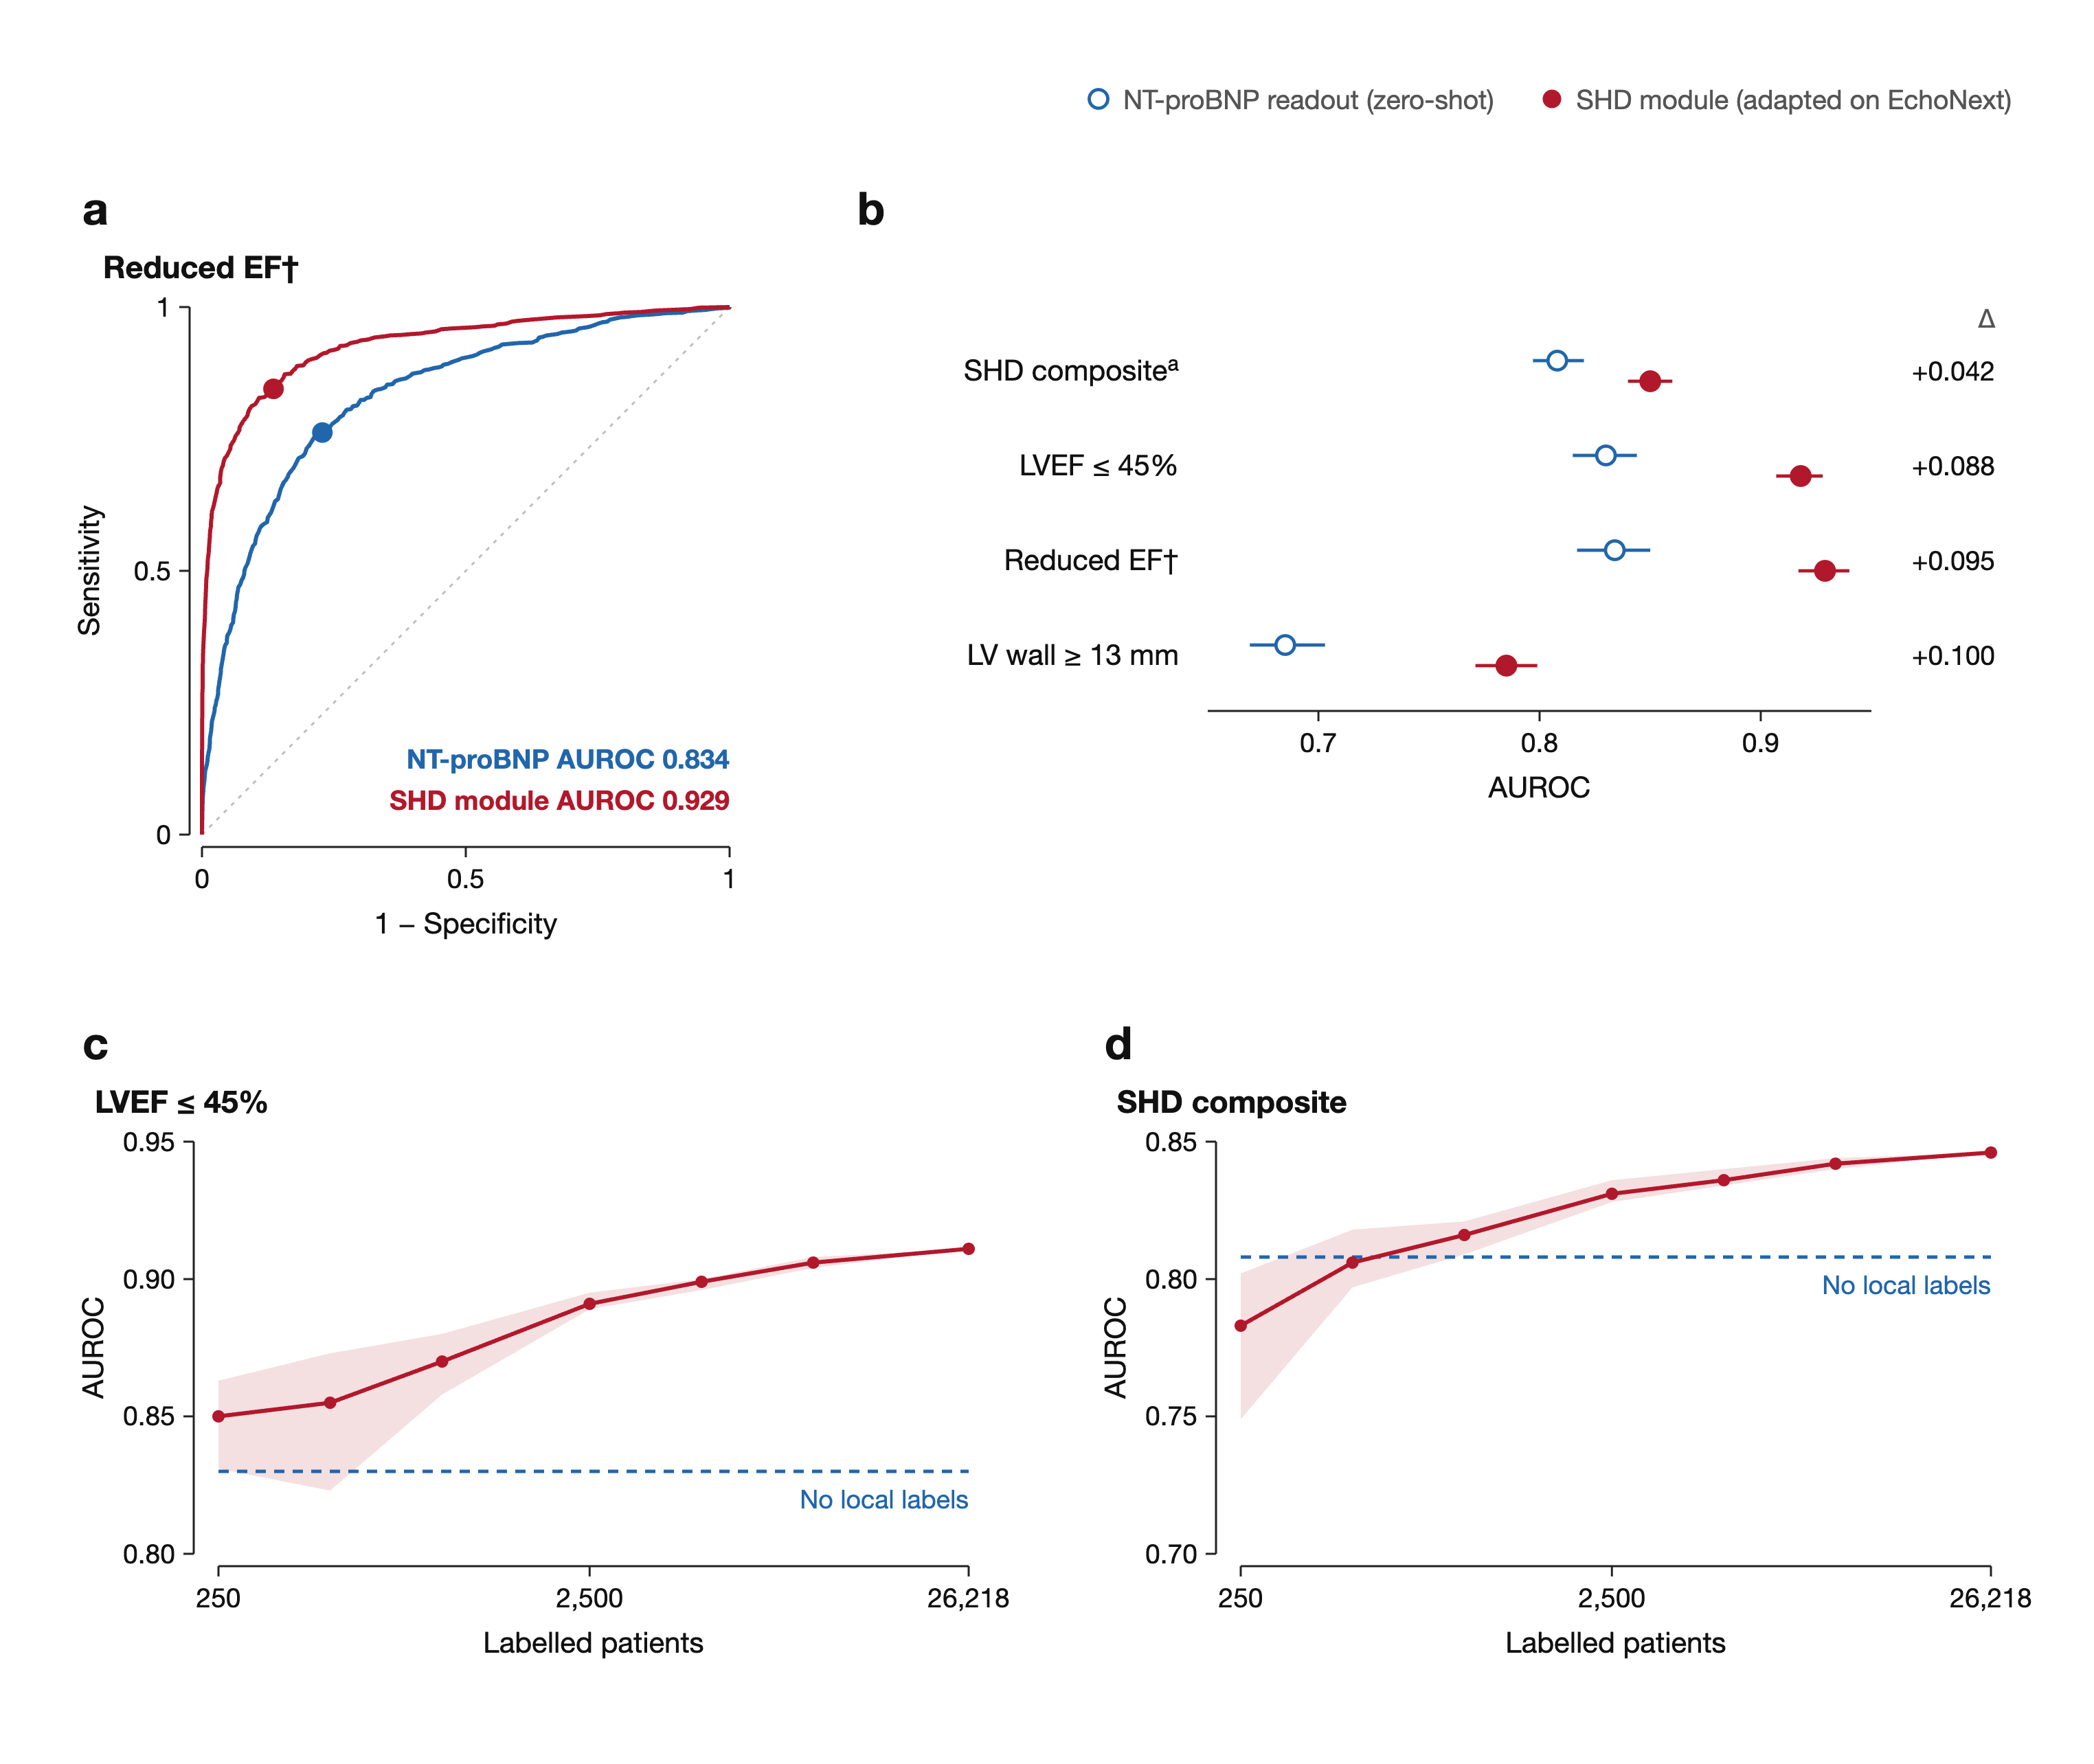
\includegraphics[width=\linewidth]{harvi_fig4_shd.png}
\caption{SHD module on held-out EchoNext test patients. (a) ROC for reduced EF$^\dagger$: NT-proBNP readout (zero-shot) and SHD module (adapted on EchoNext); filled circles are Youden points chosen on the validation split. (b) AUROC (95\,\% CI) per endpoint; right column: paired $\Delta$. (c, d) AUROC of a frozen-encoder logistic-regression probe (regularisation chosen on the validation split) against the number of echo-labelled training patients (log scale); line: mean, band: min--max of 5 draws per size, except the full training set (26{,}218 patients), which is a single fit; dashed: NT-proBNP readout with no local labels. $^a$Moderate or greater echo finding. $^\dagger$Post hoc.}\label{fig:shd}\end{figure}
Adapted on EchoNext echocardiography labels (26{,}218 training patients; mean of three seeds), the SHD module outperformed the zero-shot NT-proBNP readout on every endpoint (Table~\ref{tab:echo}, Figure~\ref{fig:shd}a,b). It reached AUROC 0.929 for reduced ejection fraction, 0.918 for LVEF $\le$45\,\% (0.943 in outpatients) and 0.850 for composite structural heart disease. The largest gain was for LV wall thickness (+0.100 (+0.085 to +0.115)), the phenotype NT-proBNP reflects least.

Few labels are needed (Figure~\ref{fig:shd}c,d). A logistic-regression probe on the frozen encoder, with its regularisation chosen on the validation split, matched the zero-label NT-proBNP readout with 250 labelled patients for LVEF $\le$45\,\% and LV wall thickness and with 1{,}000 for structural heart disease, and kept improving with more labels (LVEF $\le$45\,\%: 0.911 with all training patients).

\begin{table}[t]\centering\small
\caption{EchoNext held-out test patients. AUROC with 95\,\% patient-bootstrap CI and paired difference (SHD module $-$ NT-proBNP readout). $^a$Composite of moderate-or-greater echo findings. $^b$Post hoc endpoint.}\label{tab:echo}
\setlength\tabcolsep{4pt}\footnotesize
\begin{tabular}{lrccc}\toprule
Endpoint & Cases / $n$ & \makecell{NT-proBNP\\readout} & \makecell{SHD\\module} & $\Delta$ \\\midrule
Structural heart disease$^a$ & 2{,}318 / 5{,}442 & \makecell{0.808\\ {\scriptsize 0.796--0.820}} & \makecell{\textbf{0.850}\\ {\scriptsize 0.840--0.860}} & \makecell{+0.042\\ {\scriptsize +0.034 to +0.049}} \\ \addlinespace[2pt]
LVEF $\le$45\,\% & 962 / 5{,}442 & \makecell{0.830\\ {\scriptsize 0.816--0.844}} & \makecell{\textbf{0.918}\\ {\scriptsize 0.907--0.928}} & \makecell{+0.088\\ {\scriptsize +0.076 to +0.099}} \\ \addlinespace[2pt]
LVEF $\le$40 vs $\ge$50\,\%$^b$ & 761 / 4{,}492 & \makecell{0.834\\ {\scriptsize 0.819--0.849}} & \makecell{\textbf{0.929}\\ {\scriptsize 0.917--0.940}} & \makecell{+0.095\\ {\scriptsize +0.082 to +0.108}} \\ \addlinespace[2pt]
LV wall $\ge$13\,mm & 1{,}061 / 5{,}442 & \makecell{0.685\\ {\scriptsize 0.667--0.702}} & \makecell{\textbf{0.785}\\ {\scriptsize 0.771--0.799}} & \makecell{+0.100\\ {\scriptsize +0.085 to +0.115}} \\ \addlinespace[2pt]
\bottomrule\end{tabular}\end{table}

The two readouts are complementary: the NT-proBNP readout works at a new site without local labels, and a few hundred echo-labelled patients enable a dedicated structural heart disease screener.

\section{Operating points}\label{sec:ops}
\begin{figure}[t]\centering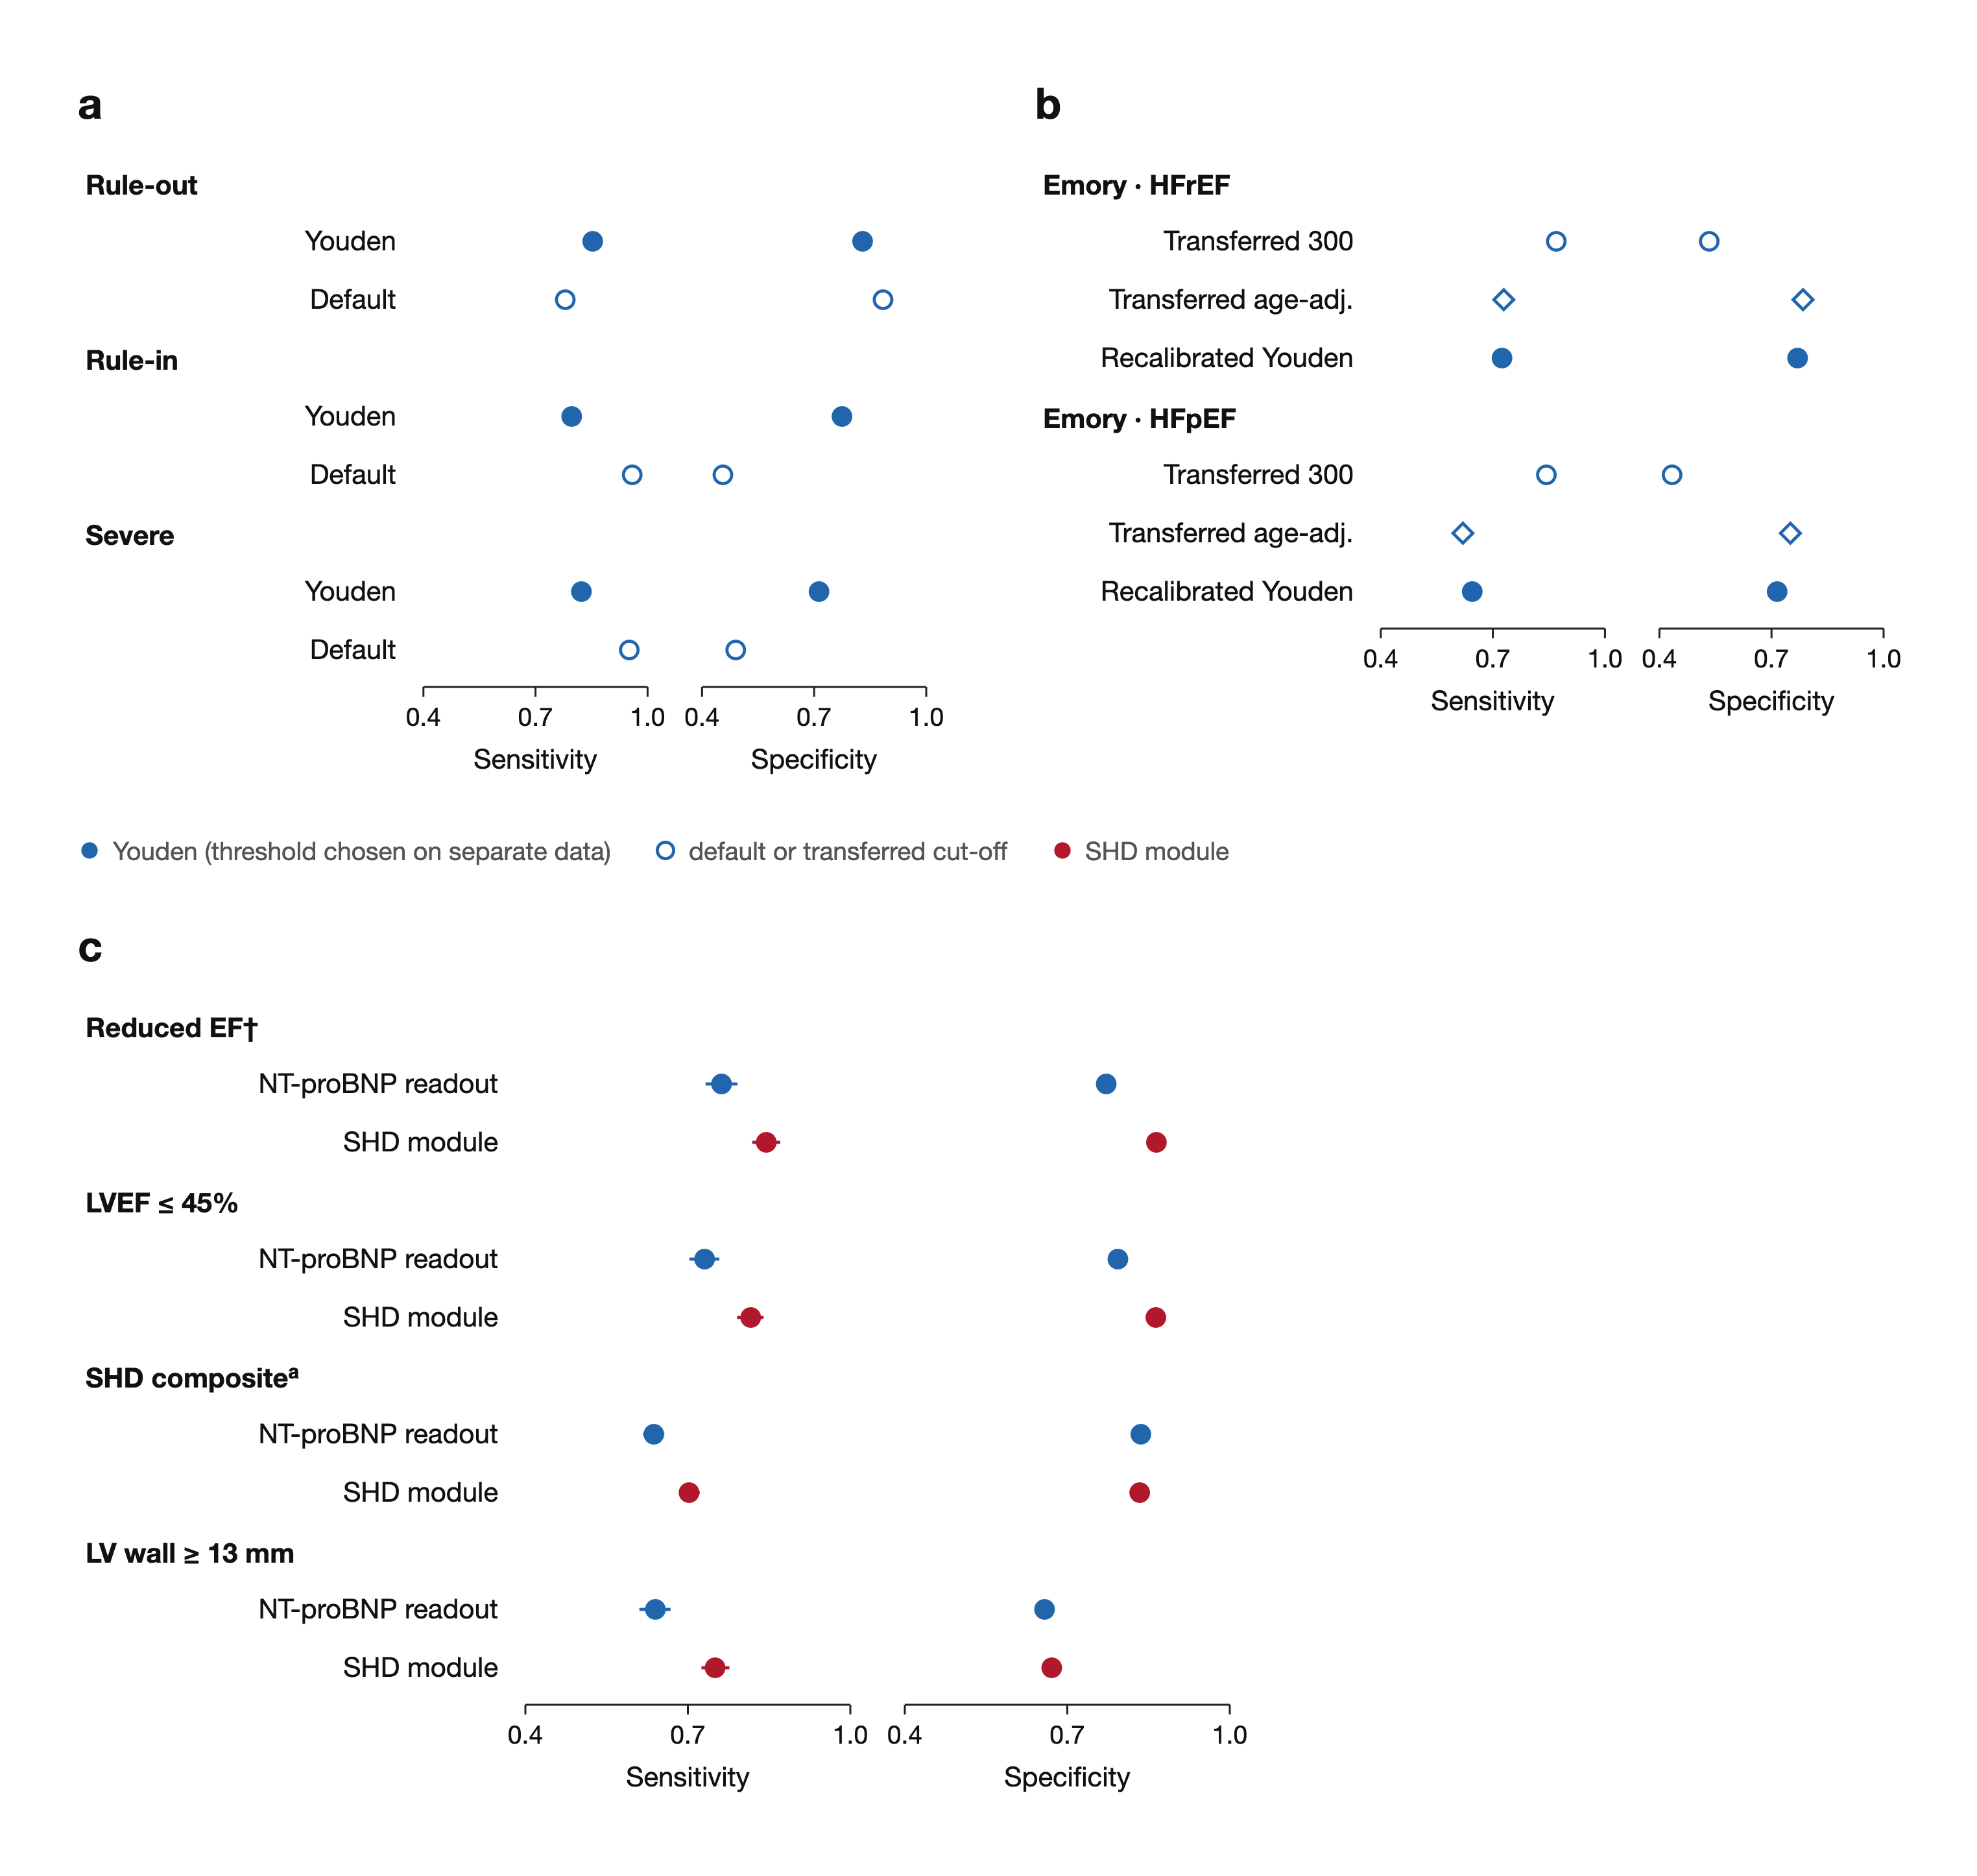
\includegraphics[width=0.92\linewidth]{harvi_fig5_operating_points.png}
\caption{Sensitivity and specificity at operating points (95\,\% CI, patient bootstrap, threshold fixed). (a) MIMIC-IV: cross-fitted Youden threshold (filled) and default threshold (open). (b) Emory: MIMIC-IV cut-offs transferred unchanged (open circle: 300\,pg/mL; open diamond: age-adjusted rule-in) and a Youden threshold recalibrated at Emory (filled). (c) EchoNext test: Youden thresholds chosen on the validation split, for both readouts. Values are listed in Table~\ref{tab:ops} (Appendix~\ref{app:ops}). $^a$Moderate or greater echo finding. $^\dagger$Post hoc.}\label{fig:ops}\end{figure}
Each threshold was chosen on data separate from the patients on which it is evaluated: in MIMIC-IV by cross-fitting (the Youden threshold of the other four folds, applied to the held-out fold), at Emory by splitting the patients into halves (Youden threshold from one half applied to the other; median of 20 repeats), and at EchoNext on the validation split. Confidence intervals come from 2{,}000 patient-bootstrap draws with the threshold held fixed.

In MIMIC-IV, the Youden thresholds give balanced sensitivity and specificity for all three decisions (rule-out 0.85/0.83, rule-in 0.80/0.77, severe 0.82/0.71; Figure~\ref{fig:ops}a), whereas the default threshold favours sensitivity for rule-in and severe. At Emory, the age-adjusted rule-in cut-offs transferred from MIMIC-IV performed as well as a threshold recalibrated at Emory itself (HFrEF 0.73/0.78 versus 0.72/0.77; Figure~\ref{fig:ops}b). The fixed 300\,pg/mL rule-out cut-off flagged most patients at Emory (specificity 0.53 for HFrEF and 0.43 for HFpEF) and is the cut-off that needs local recalibration. On EchoNext, at validation-chosen thresholds, the SHD module reached sensitivity/specificity 0.84/0.86 for reduced ejection fraction, against 0.76/0.77 for the NT-proBNP readout (Figure~\ref{fig:ops}c).

\section{Comparison with published models}\label{sec:bench}
\begin{figure}[h]\centering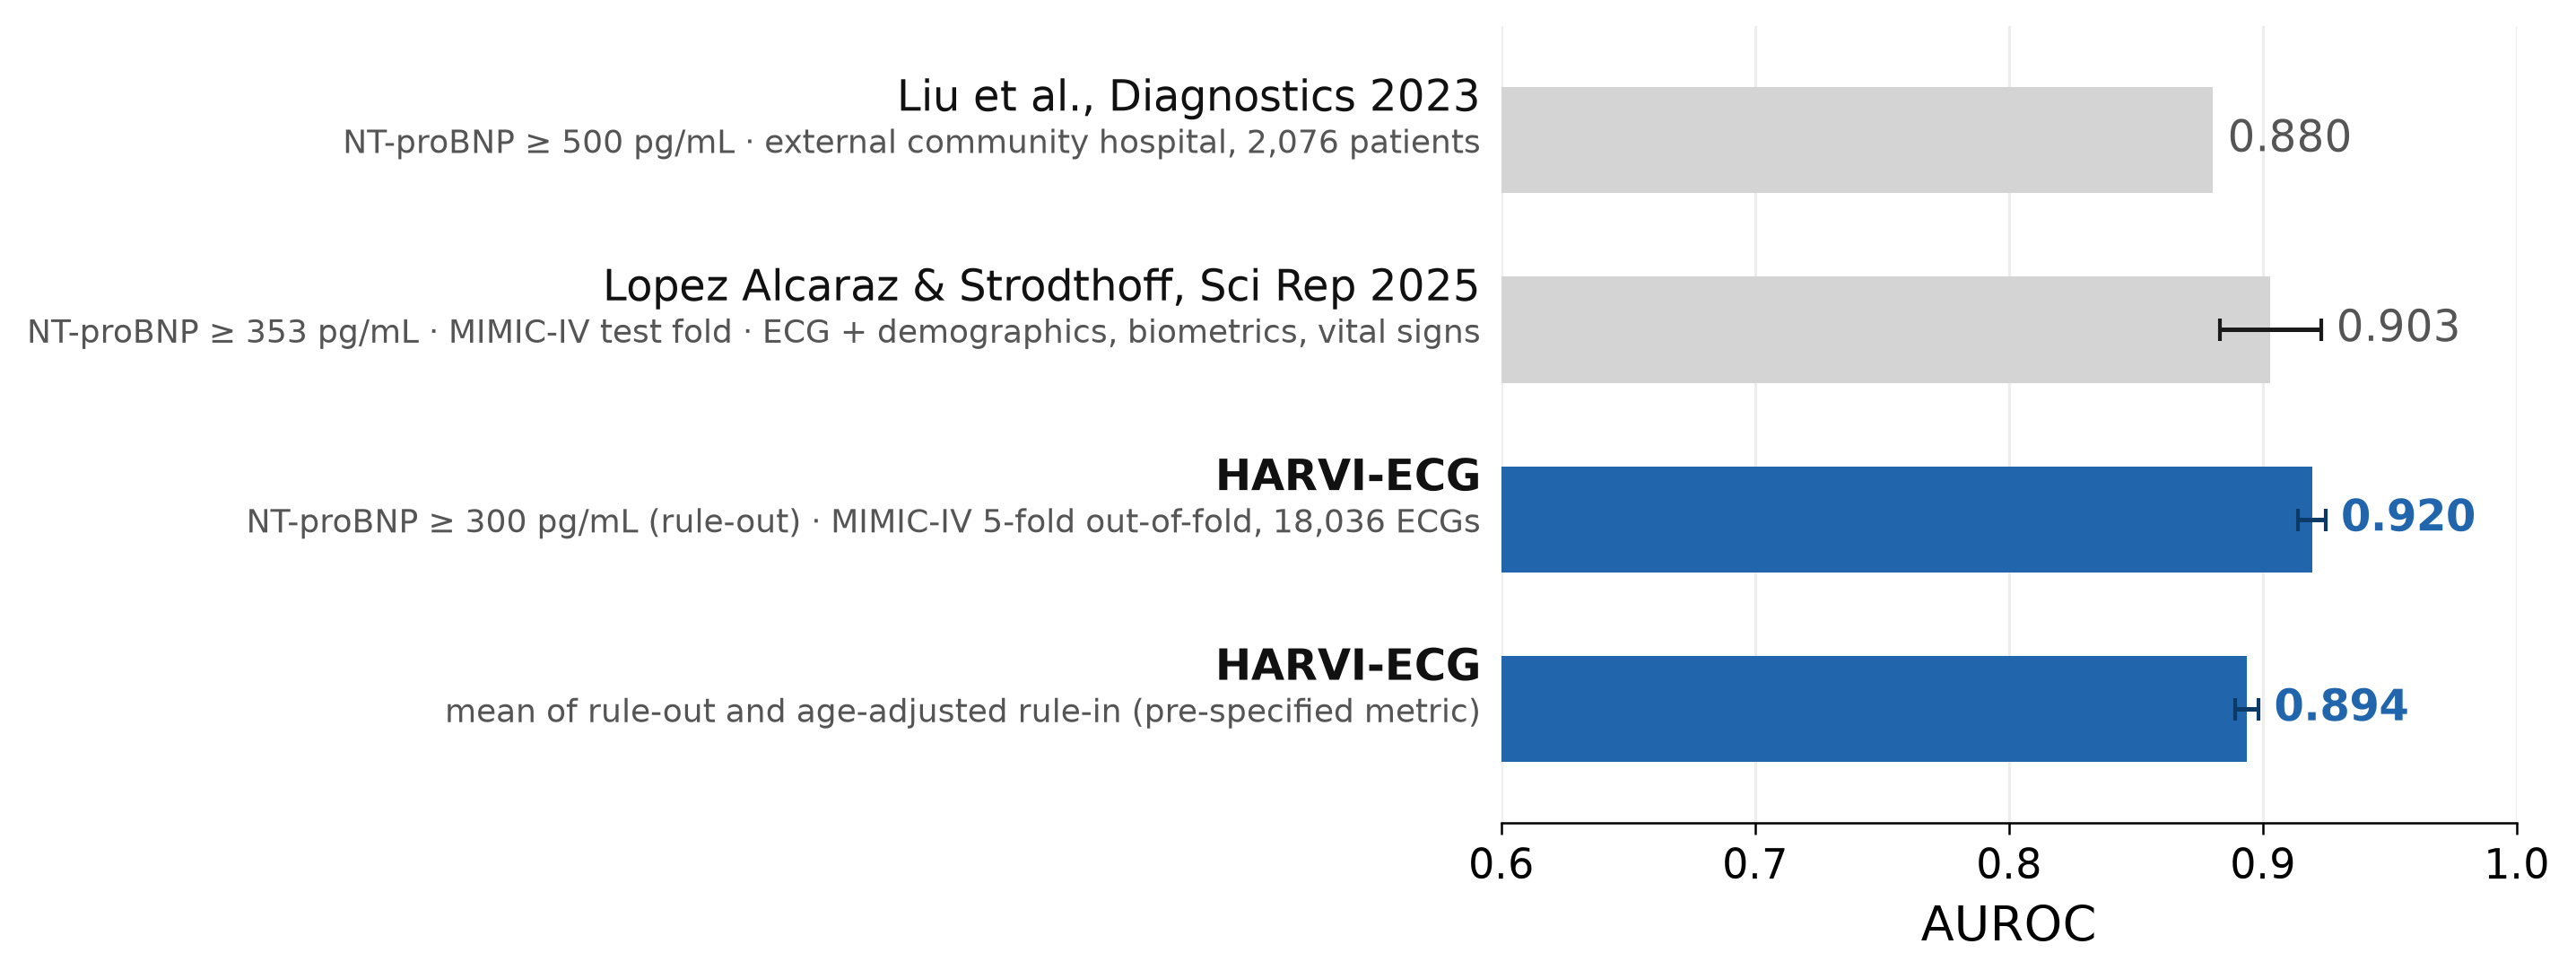
\includegraphics[width=\linewidth]{harvi_benchmark.png}
\caption{HARVI-ECG against published ECG-to-NT-proBNP models. Published values as reported: Liu et al.~\cite{liu2023}, NT-proBNP $\geq$500\,pg/mL in their external community-hospital set (AUC 0.880; 0.879 at $\geq$1{,}000\,pg/mL; no CI reported); Lopez Alcaraz and Strodthoff~\cite{lopezalcaraz2025}, NT-proBNP $\geq$353\,pg/mL on a MIMIC-IV test fold from the ECG with demographics, biometrics and vital signs (0.903, 95\,\% CI 0.883--0.923). HARVI-ECG: MIMIC-IV out-of-fold, 95\,\% patient-bootstrap CI. Thresholds, cohorts and inputs differ between studies, so the values are not a head-to-head comparison; the axis starts at 0.6.}\label{fig:bench}\end{figure}
HARVI-ECG is on par with published ECG-to-NT-proBNP models (Figure~\ref{fig:bench}). Its rule-out AUROC (0.920 (0.914--0.925); detection of NT-proBNP $\geq$300\,pg/mL) is comparable to the 0.880 reported by Liu et al.~\cite{liu2023} at their external hospital for $\geq$500\,pg/mL, and to the 0.903 reported by Lopez Alcaraz and Strodthoff~\cite{lopezalcaraz2025} for $\geq$353\,pg/mL in MIMIC-IV, which additionally used vital signs and biometrics. HARVI-ECG additionally provides zero-shot validation at two unseen hospitals and a structural heart disease readout.

\section{Limitations}\label{sec:lim}
\begin{enumerate}
\item Retrospective evaluation; prospective validation of the screening pathway is planned.
\item Emory phenotypes are ICD-10 based. EchoNext records echo findings but not symptoms, so its positives include symptomatic heart failure as well as asymptomatic structural disease (Stage B).
\item The 300\,pg/mL rule-out cut-off requires site recalibration (Section~\ref{sec:ops}). The NT-proBNP regression head was trained on the raw pg/mL scale (the pre-specification described a log scale); a log-scale head is planned. The decision rule uses the classification outputs and is unaffected.
\item Each fold model of the NT-proBNP readout was trained with a single seed.
\end{enumerate}

\section{Availability}\label{sec:avail}
Analysis code, aggregate results and figures are available in the accompanying repository and Zenodo record. Model weights (encoder, NT-proBNP readout and SHD module) are available upon reasonable request through a gated Hugging Face repository, \url{https://huggingface.co/maxhaberbusch/HARVI-ECG}; access requests are reviewed individually. The weights are licensed under the HARVI-ECG Model Weights Research Licence (non-commercial research only, no clinical use, no redistribution); HARVI-ECG is not a medical device. MIMIC-IV and HEEDB are credentialed-access datasets and EchoNext is available under its data-use agreement; patient-level data and predictions are not redistributed.

\begin{thebibliography}{9}\small\setlength{\itemsep}{1pt}
\bibitem{gow2023} B.~Gow, T.~Pollard, L.~A. Nathanson, et~al. MIMIC-IV-ECG: diagnostic electrocardiogram matched subset (version 1.0). \emph{PhysioNet}, 2023. doi:10.13026/4nqg-sb35.
\bibitem{johnson2023} A.~E.~W. Johnson, L.~Bulgarelli, L.~Shen, et~al. MIMIC-IV, a freely accessible electronic health record dataset. \emph{Scientific Data}, 10:1, 2023.
\bibitem{koscova2026} Z.~Koscova, Q.~Li, C.~Robichaux, et~al. The Harvard-Emory ECG Database. \emph{Scientific Data}, 13:516, 2026. doi:10.1038/s41597-026-06861-9.
\bibitem{beck2024} M.~Beck, K.~P\"oppel, M.~Spanring, et~al. xLSTM: Extended long short-term memory. In \emph{Advances in Neural Information Processing Systems (NeurIPS)}, 2024. arXiv:2405.04517.
\bibitem{liu2023} P.-Y. Liu, C.~Lin, C.-S. Lin, W.-H. Fang, C.-C. Lee, C.-H. Wang, and D.-J. Tsai. Artificial intelligence-enabled electrocardiography detects B-type natriuretic peptide and N-terminal pro-brain natriuretic peptide. \emph{Diagnostics}, 13(17):2723, 2023. doi:10.3390/diagnostics13172723.
\bibitem{lopezalcaraz2025} J.~M. Lopez Alcaraz and N.~Strodthoff. Abnormality prediction and forecasting of laboratory values from electrocardiogram signals using multimodal deep learning. \emph{Scientific Reports}, 15:39362, 2025. doi:10.1038/s41598-025-26715-5.
\bibitem{hu2022} E.~J. Hu, Y.~Shen, P.~Wallis, et~al. LoRA: Low-rank adaptation of large language models. In \emph{International Conference on Learning Representations (ICLR)}, 2022. arXiv:2106.09685.
\end{thebibliography}

\appendix
\section{Operating points}\label{app:ops}
\begin{table}[h]\centering\footnotesize\setlength{\tabcolsep}{4pt}
\caption{Operating points (values shown in Figure~\ref{fig:ops}). Sensitivity and specificity with 95\,\% CI (2{,}000 patient-bootstrap draws, threshold fixed). MIMIC-IV probability thresholds are the median of the five fold thresholds. For rule-out, the positive class is measured NT-proBNP $<$300\,pg/mL. $^a$Moderate or greater echo finding. $^\dagger$LVEF $\le$40\,\% vs $\ge$50\,\%, post hoc.}\label{tab:ops}
\begin{tabular}{@{}llcc@{}}\toprule
Operating point & Threshold & Sensitivity & Specificity \\\midrule
\multicolumn{4}{@{}l}{\textit{MIMIC-IV, out-of-fold (NT-proBNP readout)}} \\
\quad Rule-out, Youden (cross-fitted) & $p \geq 0.33$ & 0.85 (0.84--0.87) & 0.83 (0.82--0.84) \\
\quad Rule-out, default & $p \geq 0.50$ & 0.78 (0.76--0.80) & 0.88 (0.88--0.89) \\
\quad Rule-in, Youden (cross-fitted) & $p \geq 0.89$ & 0.80 (0.79--0.81) & 0.77 (0.76--0.79) \\
\quad Rule-in, default & $p \geq 0.50$ & 0.96 (0.95--0.96) & 0.46 (0.44--0.47) \\
\quad Severe, Youden (cross-fitted) & $p \geq 0.84$ & 0.82 (0.81--0.83) & 0.71 (0.70--0.72) \\
\quad Severe, default & $p \geq 0.50$ & 0.95 (0.95--0.96) & 0.49 (0.48--0.50) \\
\addlinespace
\multicolumn{4}{@{}l}{\textit{Emory, zero-shot (NT-proBNP readout)}} \\
\quad HFrEF, transferred 300 pg/mL & 300 pg/mL & 0.87 (0.86--0.88) & 0.53 (0.53--0.54) \\
\quad HFrEF, transferred age-adjusted rule-in & 450/900/1{,}800 pg/mL & 0.73 (0.72--0.74) & 0.78 (0.78--0.79) \\
\quad HFrEF, recalibrated Youden & 992 pg/mL & 0.72 (0.71--0.74) & 0.77 (0.76--0.78) \\
\quad HFpEF, transferred 300 pg/mL & 300 pg/mL & 0.84 (0.83--0.85) & 0.43 (0.43--0.44) \\
\quad HFpEF, transferred age-adjusted rule-in & 450/900/1{,}800 pg/mL & 0.62 (0.61--0.63) & 0.75 (0.74--0.76) \\
\quad HFpEF, recalibrated Youden & 1{,}057 pg/mL & 0.64 (0.63--0.66) & 0.71 (0.71--0.72) \\
\addlinespace
\multicolumn{4}{@{}l}{\textit{EchoNext, held-out test (Youden threshold from the validation split)}} \\
\quad Reduced EF$^\dagger$, NT-proBNP readout & 2{,}203 pg/mL & 0.76 (0.73--0.79) & 0.77 (0.76--0.79) \\
\quad Reduced EF$^\dagger$, SHD module & $p \geq 0.25$ & 0.84 (0.82--0.87) & 0.86 (0.85--0.88) \\
\quad LVEF $\le$45\,\%, NT-proBNP readout & 2{,}203 pg/mL & 0.73 (0.70--0.76) & 0.79 (0.78--0.80) \\
\quad LVEF $\le$45\,\%, SHD module & $p \geq 0.24$ & 0.82 (0.79--0.84) & 0.86 (0.85--0.87) \\
\quad SHD composite$^a$, NT-proBNP readout & 1{,}406 pg/mL & 0.64 (0.62--0.66) & 0.84 (0.82--0.85) \\
\quad SHD composite$^a$, SHD module & $p \geq 0.53$ & 0.70 (0.68--0.72) & 0.83 (0.82--0.85) \\
\quad LV wall $\ge$13\,mm, NT-proBNP readout & 1{,}155 pg/mL & 0.64 (0.61--0.67) & 0.66 (0.64--0.67) \\
\quad LV wall $\ge$13\,mm, SHD module & $p \geq 0.20$ & 0.75 (0.73--0.78) & 0.67 (0.66--0.68) \\
\bottomrule\end{tabular}\end{table}
\end{document}
